\documentclass[conference]{IEEEtran}
\usepackage[T1]{fontenc}
\usepackage{amsmath,amssymb}
\usepackage{graphicx}
\usepackage{booktabs}
\usepackage{multirow}
\usepackage{xcolor}
\usepackage[hidelinks]{hyperref}
\usepackage{cite}
\newcommand{\JS}{J_{\mathrm{sup}}}
\newcommand{\JR}{J_{\mathrm{rec}}}
\newcommand{\add}{\textsc{add}}
\newcommand{\rem}{\textsc{remove}}
\newcommand{\stp}{\textsc{stop}}

\begin{document}

\title{Learning to Add, Remove and Swap:\\ Reversible Reinforcement Learning for\\ Excitation--Emission Pair Selection}

% TODO(authors): confirm author list and affiliations (student co-author who wrote the formulation).
\author{\IEEEauthorblockN{[Author names]}
\IEEEauthorblockA{\textit{[Affiliations]}}}

\maketitle

\begin{abstract}
Selecting a few excitation--emission pairs from a multi-excitation fluorescence image is a fixed-budget combinatorial problem in which the value of a pair depends on the pairs already chosen. Constructive reinforcement-learning (RL) policies can only add, so early mistakes are permanent. We formulate pair selection as a reversible Markov decision process with add, remove and stop actions, paired credit for each remove--add swap, tabu masking, and a permutation-invariant candidate scorer built on label-free residual-variance features, so that one policy applies to datasets with different candidate sets. On four annotated datasets (two lichen, two collagen) with nested, specimen-grouped evaluation we separate three regimes. On a single labelled dataset RL is a weak black-box optimiser: simulated annealing and a genetic algorithm reach the exact optimum at $n=3$ and higher objective values at a matched budget. Deployed \emph{without labels} on an unseen sample type, the reversible policy beats a matched add-only policy by $+0.025$ balanced accuracy (95\% CI $[0.022,0.028]$; significant for all four variants), the gain is largest across sample families, and the reversible policy is not harder to train. A label-free greedy baseline nevertheless remains hard to beat at small budgets, and using the swap policy to refine that greedy set helps on one target but usually leaves it unchanged. With 25 labelled evaluations, transferred policies match simulated annealing, which overtakes them at larger budgets.
\end{abstract}

\begin{IEEEkeywords}
band selection, reinforcement learning, fluorescence, hyperspectral imaging, combinatorial optimisation
\end{IEEEkeywords}

%=====================================================================
\section{Introduction}
Multi-excitation fluorescence hyperspectral imaging records, for every pixel, an excitation--emission matrix (EEM): the sample is illuminated at several excitation wavelengths $\lambda^{\mathrm{ex}}$ and a full emission spectrum is recorded at each~\cite{lakowicz2006}. One measurement channel is therefore a \emph{pair} $c=(\lambda^{\mathrm{ex}},\lambda^{\mathrm{em}})$, and an acquisition yields 150--210 admissible pairs after Rayleigh-scatter rejection. Measuring all of them is slow, photobleaches the sample and needs a tunable source; a handful of well-chosen pairs would allow a cheap instrument with a few LEDs and fixed filters. Choosing $n$ of $M$ pairs is a combinatorial problem ($\binom{192}{13}\approx5\times10^{19}$), and the value of a pair depends on the pairs already chosen.

Reinforcement learning (RL) is attractive for such sequential set construction~\cite{bello2016,khalil2017,kool2019}, and has been applied to hyperspectral band selection~\cite{mou2022drl}. Constructive policies, however, can only \emph{add}: an early mistake is permanent. In combinatorial RL, reversible actions that also remove elements improved solution quality~\cite{barrett2020eco,chen2019rewriting}. We ask whether the same holds for spectral pair selection, and, crucially, \emph{where} RL can add value at all. Our contributions are:
\begin{itemize}
\item a reversible add/remove/stop MDP for fixed-budget pair selection with paired credit assignment, tabu masking and a permutation-invariant candidate scorer that transfers across datasets with different candidate sets;
\item a protocol that separates three regimes---per-instance search at a matched evaluation budget, label-free transfer to an unseen dataset, and few-shot search with a small labelled budget---with nested, specimen-grouped evaluation;
\item a study on four labelled fluorescence datasets (two lichen, two collagen) against classic search (greedy, swap, beam, simulated annealing, genetic), exact small-budget optima and label-free baselines.
\end{itemize}
We find that reversibility helps exactly where RL is used beyond a single instance---on new data---while classic search remains the better optimiser of a fixed objective.

%=====================================================================
\section{Problem}
Let $\mathcal{C}=\{c_j\}_{j=1}^{M}$ be the admissible pairs (first- and second-order Rayleigh bands removed). Pixels $x_i\in\mathbb{R}^M$ carry a class $y_i$ and a specimen id $g_i$. For a budget $n$ we seek
\begin{equation}
S^\star=\arg\max_{S\subset\mathcal{C},\,|S|=n} \mathrm{BA}_{\mathrm{test}}(S),
\end{equation}
the balanced accuracy of a classifier trained on the selected pairs and tested on \emph{specimens not used for selection}. The search can only use a surrogate computed on training specimens. We use two:
\textbf{Supervised} $\JS(S)$: the balanced accuracy of shrinkage LDA under inner whole-specimen cross-validation. Per inner fold we precompute class sums and the pooled within-class scatter for all $M$ pairs once; scoring any $S$ is then a $|S|\times|S|$ submatrix solve ($\approx0.5$\,ms), which makes RL training with $10^5$--$10^6$ evaluations feasible.
\textbf{Label-free} $\JR(S)=\mathrm{tr}(\Sigma_{:S}\Sigma_{SS}^{-1}\Sigma_{S:})/\mathrm{tr}\,\Sigma$: the fraction of variance of all $M$ standardised pairs that is linearly predictable from $S$ (column-subset selection~\cite{boutsidis2009css}), computable on a new, unlabelled sample.
Labels are expensive and absent for new samples, so a method meant for new data must act label-free; $\JS$ is available only on annotated training datasets.

%=====================================================================
\section{Reversible selection MDP}
\textbf{State and actions.} The state is the current set $S_t$, a phase $q_t\in\{\add,\rem\}$ and a tabu list. Episodes start from $S_0=\emptyset$ (or from a label-free greedy set) and \emph{construct} by \add{} until $|S|=n$. In \emph{add/remove} mode they then run up to $T=n$ refinement cycles: the agent either \stp{}s or removes a pair $c_r\in S$, after which only an \add{} of $c_a\notin S$ is allowed, so every cycle is a learned swap $S'=(S\setminus\{c_r\})\cup\{c_a\}$ that preserves the budget. Masks forbid duplicates, invalid pairs, re-adding a removed pair for $L=3$ cycles and removing the pair just added; revisiting a subset costs $-0.01$.
\textbf{Reward.} Construction steps receive $r_t=J(S_{t+1})-J(S_t)$ with $J(\emptyset)$ at chance. A removal receives $0$ and the following addition $J(S')-J(S)$, so both halves of a swap share the credit of the completed replacement and the return telescopes to $J(S_{\mathrm{final}})-J(\emptyset)$.
\textbf{Candidate features.} Each pair $c$ is described, given $S$, by label-free quantities standardised within the task: wavelengths and Stokes shift, log-intensity mean and spread, residual variance of $c$ given $S$, the gain in $\JR$ (and in a whitened-PCA variant) if $c$ is added or the loss if it is removed---all from rank-one updates of the residual covariance---maximum and mean $|\mathrm{corr}|$ with $S$, and excitation-sharing indicators. Optional supervised features (Fisher score, exact pair-enumeration priors) are used only when labels are available.
\textbf{Policy.} A shared MLP embeds every candidate; the set context is the mean and max of the selected embeddings plus global features (phase, $|S|/n$, current $\JR$)~\cite{zaheer2017deepsets}. Separate \add{} and \rem{} heads score candidates, a \stp{} head and a value head read the context; logits are masked. The policy ($\approx$38k parameters) never sees a pair index, so it applies to any candidate set. We train with PPO~\cite{schulman2017ppo} on batches of 64 episodes sampled over tasks and budgets $n\in\{3,5,8,13\}$, masking a random 20\% of pairs as augmentation; REINFORCE~\cite{williams1992} is an ablation.
\textbf{Deployment.} Label-free: a greedy rollout, or the best of 16 sampled rollouts ranked by $\JR$; no labels and no $\JS$ calls, and the \emph{final} set is returned. Few-shot ($\JS$ observable, budget $B$): best-of-$k$ sampling for add-only, and Monte-Carlo look-ahead for add/remove, which evaluates the top removals with sampled replacements and applies the best improving swap.

%=====================================================================
\section{Experimental protocol}
\textbf{Data.} Four annotated multi-excitation fluorescence datasets acquired with a tunable source and a liquid-crystal tunable filter (emission 420--720\,nm in 10\,nm steps): \emph{Lichens1} (1040$\times$925\,px, 8 excitations 310--430\,nm, $M=192$, 4 classes, 16 specimens, public~\cite{lichens_zenodo}), \emph{Lichens2} (the same lichens at camera resolution with different processing, $M=210$, 5 classes, 28 specimens), and two collagen digestion series, \emph{Collagen-AA} (acetic acid, $M=149$) and \emph{Collagen-P} (pepsin, $M=158$), each with 3 classes and 9 specimens. A specimen is a connected annotated region; it is the unit of independence.
\textbf{Nested, specimen-grouped evaluation.} Outer folds hold out at least one whole specimen per class (k = 4, 2, 3, 3 folds; three seeded repeats)~\cite{roberts2017cv,varma2006bias}. Every selection method sees only the training specimens; $\JS$ uses inner whole-specimen folds on a per-specimen capped subsample ($\approx$3000 px). Selected sets are scored on the held-out specimens by kNN ($k=5$, primary, as in our earlier work), shrinkage LDA, an RBF-SVM and a random forest; we report balanced accuracy (BA) and macro-F1, the number of distinct excitations, mean $|\mathrm{corr}|$, and selection stability (Kuncheva index~\cite{kuncheva2007stability}).
\textbf{Methods.} Label-free: random (10 draws), top variance, a uniform excitation--emission grid, SPA~\cite{araujo2001spa}, greedy $\JR$ (column-subset greedy, CSS) and its whitened-PCA variant, and a variance-relevance/correlation-penalty rule mimicking our earlier selector. Supervised filters: Fisher score and mRMR~\cite{peng2005mrmr}. Wrapper search on $\JS$ with a budget of $B$ uncached evaluations: random search, sequential forward selection (SFS), SFS followed by best-improvement swaps, beam search (width 5) with swaps, simulated annealing (SA)~\cite{kirkpatrick1983sa}, a steady-state genetic algorithm (GA), and exact enumeration for $n\le3$.
\textbf{Regimes.} \emph{S1 search:} all wrappers and per-instance RL on each training task, $B=5000$, best-so-far set. \emph{S2 transfer:} policies trained with $\JS$ reward on the source datasets---leave-one-dataset-out (LODO) and cross-family (Lichens$\rightarrow$Collagen, Collagen$\rightarrow$Lichens)---and deployed label-free on every outer fold of the target. \emph{S3 few-shot:} the transferred policy with $\JS$ observable on the target and $B\in\{25,\dots,400\}$. Budgets $n\in\{3,5,8,13\}$ throughout.

\section{Results}
\begin{figure*}[t]
\centering
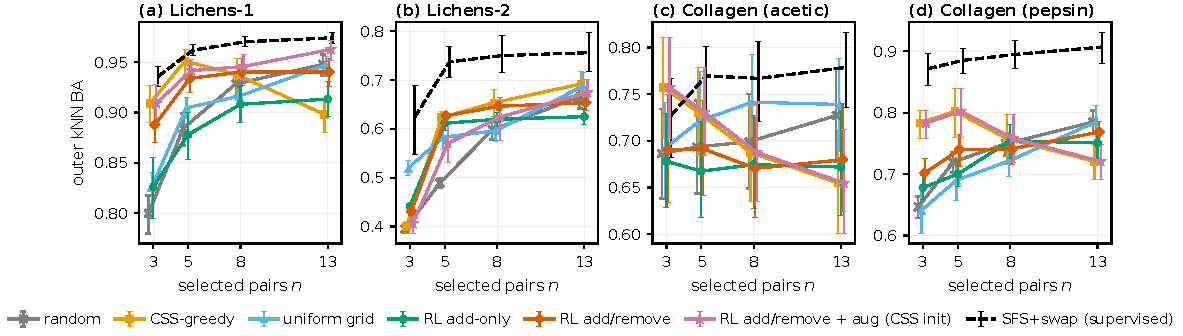
\includegraphics[width=\textwidth]{figures/fig_transfer.pdf}
\caption{Label-free transfer to an unseen sample type (S2). Policies are trained with $\JS$ reward on the other family (Collagen$\rightarrow$Lichens for (a,b), Lichens$\rightarrow$Collagen for (c,d)) and deployed without labels (best of 16 rollouts ranked by $\JR$). Outer-test kNN balanced accuracy, mean and 95\% bootstrap CI over 3 repeats $\times$ outer folds. Dashed: supervised SFS+swap on the target (upper reference).}
\label{fig:transfer}
\end{figure*}

\begin{table}[t]
\centering
\caption{Search at a matched budget (S1, $B=5000$, mean over the 4 datasets and repeat-0 folds) and ablations (Collagen-AA, $n=8$, $B=20000$, oracle cost charged). $\JS$ is the inner objective; kNN BA is on held-out specimens.}
\label{tab:search}
\resizebox{\columnwidth}{!}{{\small
\setlength{\tabcolsep}{4pt}
\begin{tabular}{lccccc}
\toprule
 & \multicolumn{2}{c}{$n=5$} & \multicolumn{2}{c}{$n=13$} & $n=3$ \\
\cmidrule(lr){2-3}\cmidrule(lr){4-5}\cmidrule(lr){6-6}
Method & $J_{\mathrm{sup}}$ & kNN BA & $J_{\mathrm{sup}}$ & kNN BA & gap to exact \\
\midrule
RL add-only & 0.864 & 0.826 & 0.883 & 0.841 & -- \\
RL add/remove & 0.861 & 0.813 & 0.887 & 0.844 & -- \\
SFS+swap & 0.871 & 0.835 & 0.916 & 0.853 & 0.009 \\
Beam+swap & 0.872 & 0.836 & 0.845 & 0.819 & 0.008 \\
SA & 0.884 & 0.838 & 0.920 & 0.856 & 0.000 \\
GA & 0.885 & 0.835 & 0.924 & 0.860 & 0.000 \\
Random search & 0.854 & 0.817 & 0.885 & 0.839 & 0.020 \\
\multicolumn{6}{l}{\scriptsize Exact optimum at $n=3$: mean $J_{\mathrm{sup}}=0.869$ (budget 5000 per method; mean over datasets).} \\
\midrule
\multicolumn{6}{l}{\emph{Ablation: collagen (acetic), $n=8$, $B=20000$, 3 outer folds}} \\
 & \multicolumn{2}{c}{$J_{\mathrm{sup}}$} & \multicolumn{2}{c}{kNN BA} & \\
RL add-only & \multicolumn{2}{c}{0.869} & \multicolumn{2}{c}{0.764} & \\
\quad + oracle prior & \multicolumn{2}{c}{0.867} & \multicolumn{2}{c}{0.759} & \\
RL add/remove & \multicolumn{2}{c}{0.870} & \multicolumn{2}{c}{0.762} & \\
\quad + oracle prior & \multicolumn{2}{c}{0.866} & \multicolumn{2}{c}{0.753} & \\
\quad terminal reward & \multicolumn{2}{c}{0.870} & \multicolumn{2}{c}{0.765} & \\
\quad REINFORCE & \multicolumn{2}{c}{0.839} & \multicolumn{2}{c}{0.736} & \\
\quad + MC look-ahead & \multicolumn{2}{c}{0.866} & \multicolumn{2}{c}{0.779} & \\
SA & \multicolumn{2}{c}{0.881} & \multicolumn{2}{c}{0.767} & \\
SFS+swap & \multicolumn{2}{c}{0.822} & \multicolumn{2}{c}{0.735} & \\
\bottomrule
\end{tabular}
}
}
\end{table}

\textbf{Per-instance search (S1, Table~\ref{tab:search}).} On a single labelled dataset RL is a black-box optimiser, and a weak one: at $B=5000$ evaluations SA and GA reach the highest inner $\JS$ (0.920/0.924 at $n=13$ versus 0.883/0.887 for add-only/add-remove RL) and recover the exact optimum at $n=3$ on every task, while SFS+swap and beam search stop $\approx$0.01 short. RL needs $\approx$2900 evaluations to come within 0.005 of its own final value (Fig.~\ref{fig:training}b). Outer-test accuracy differences between all searchers are small (0.84--0.86 at $n=13$) because the inner objective is optimistic: its gap to the outer BA is 0.04--0.06 and grows with search strength (SA/GA 0.064 at $n=13$, random search 0.046), the winner's curse of selecting on few specimens~\cite{varma2006bias}. Among RL design choices PPO is clearly better than REINFORCE (0.870 vs 0.839 inner $\JS$), exact pair-enumeration priors do not repay their 11k-evaluation cost, terminal and shaped rewards end at the same value, and Monte-Carlo look-ahead gives the best outer accuracy of all methods on Collagen-AA (0.779) at half the budget.

\textbf{Label-free transfer (S2, Fig.~\ref{fig:transfer}, Table~\ref{tab:transfer}).} This is the regime the reversible action was meant for, and the add/remove policy is consistently better than the matched add-only policy: pooled over targets, sources and budgets the gain is $+0.025$ BA (95\% CI $[0.022, 0.028]$, 837 wins/315 losses over 1152 paired units); on cell means (32 target$\times$source$\times n$ cells) it is $+0.020$ to $+0.031$ for each of the four policy/deployment variants (Holm $p\le7\times10^{-3}$, $\ge$21/32 cells). The gain is largest across sample families ($+0.024$ to $+0.045$) where the constructive policy errs most, and on Lichens1 it holds in all 12 units at every $n$ ($+0.027$ to $+0.062$). Removing the wavelength-position features improves every policy ($+0.014$ to $+0.026$, $p<10^{-5}$): absolute or relative wavelengths encode the chemistry of the source and mislead on another sample type. In absolute terms, however, a transferred policy alone rarely beats the label-free greedy CSS baseline, which is very strong at small $n$; it does at $n=13$ on Lichens1 ($+0.042$, 12/12 units). \textbf{Task augmentation and CSS refinement (S2).} To enlarge the small source pools we retrained every policy on augmented tasks (class subsets, excitation dropout; 42--105 tasks per pool, 250 instead of 400 updates, one seed). The reversible advantage replicates on these independently trained policies: add/remove beats add-only by $+0.019$ cross-family (86/58 units, $p=0.005$; $+0.023$, $p=10^{-7}$ with best-of-16) and by $+0.027$ under LODO (114/30, $p=10^{-13}$). Augmentation itself did not help (add-only $+0.002$; add/remove $-0.024$ cross-family, $p=4\times10^{-6}$, n.s.\ under LODO), although shorter training confounds this. Mixing the label-free objective into the training reward ($\Delta\JS+0.5\,\Delta\JR$) recovers $+0.013$ cross-family ($p=0.001$) but costs $0.007$ under LODO. Started from the CSS set (``+aug'', Table~\ref{tab:transfer}) the policy is a conservative refiner, not a reliable one: the collagen-trained policy edits it on the lichen targets, improving it on Lichens-1 (0.937$\rightarrow$0.946 at $n=8$, 11/12 units; 0.898$\rightarrow$0.963 at $n=13$, 12/12, above random at 0.948) but lowering it on Lichens-2 ($-0.02$ to $-0.05$ at $n\ge5$). The lichen-trained policy and every LODO policy stop at once and return CSS unchanged.

\begin{table*}[t]
\centering
\caption{Label-free transfer (S2), outer kNN BA (mean over 3 repeats $\times$ folds). RL columns: wavelength-free features, best of 16 rollouts by $\JR$, cross-family source. ``+aug'': trained with class-subset and excitation-dropout task augmentation, refining the CSS set (identical to CSS where the policy stops at once). $p_{\mathrm{add}}$: Holm-corrected Wilcoxon $p$ of add/remove vs add-only (sign = direction); $p_{\mathrm{CSS}}$: add/remove vs CSS. $^{*}p<0.05$. Bold: best label-free value.}
\label{tab:transfer}
{\small
\setlength{\tabcolsep}{3pt}
\begin{tabular}{llccccccrr}
\toprule
Target & $n$ & Random & CSS & Best other & RL add & RL add/rem & RL +aug & $p_{\mathrm{add}}$ & $p_{\mathrm{CSS}}$ \\
\midrule
Lichens 1 & 3 & 0.800 & \textbf{0.909} & 0.826\,{\scriptsize(grid)} & 0.826 & 0.888 & \textbf{0.909} & $+$.012$^{*}$ & $-$.012$^{*}$ \\
 & 8 & 0.928 & 0.937 & 0.916\,{\scriptsize(grid)} & 0.908 & 0.940 & \textbf{0.946} & $+$.012$^{*}$ & $+$1.00 \\
 & 13 & 0.948 & 0.898 & 0.947\,{\scriptsize(grid)} & 0.913 & 0.940 & \textbf{0.963} & $+$.012$^{*}$ & $+$.012$^{*}$ \\
\midrule
Lichens 2 & 3 & 0.395 & 0.400 & \textbf{0.519}\,{\scriptsize(grid)} & 0.442 & 0.431 & 0.406 & $-$.625 & $+$.438 \\
 & 8 & 0.598 & \textbf{0.653} & 0.596\,{\scriptsize(grid)} & 0.620 & 0.646 & 0.624 & $+$.438 & $-$1.00 \\
 & 13 & 0.665 & \textbf{0.692} & 0.687\,{\scriptsize(grid)} & 0.625 & 0.654 & 0.675 & $+$.438 & $-$1.00 \\
\midrule
Collagen-AA & 3 & 0.686 & \textbf{0.757} & 0.746\,{\scriptsize(var)} & 0.678 & 0.690 & \textbf{0.757} & $+$1.00 & $-$.074 \\
 & 8 & 0.699 & 0.688 & \textbf{0.743}\,{\scriptsize(var)} & 0.674 & 0.670 & 0.688 & $-$1.00 & $-$1.00 \\
 & 13 & 0.727 & 0.655 & \textbf{0.743}\,{\scriptsize(var)} & 0.672 & 0.680 & 0.655 & $+$.141 & $+$.188 \\
\midrule
Collagen-P & 3 & 0.647 & \textbf{0.783} & 0.641\,{\scriptsize(grid)} & 0.678 & 0.702 & \textbf{0.783} & $+$.602 & $-$.141 \\
 & 8 & 0.749 & \textbf{0.758} & 0.721\,{\scriptsize(grid)} & 0.754 & 0.741 & \textbf{0.758} & $-$1.00 & $-$1.00 \\
 & 13 & \textbf{0.785} & 0.721 & \textbf{0.785}\,{\scriptsize(grid)} & 0.751 & 0.768 & 0.721 & $+$1.00 & $+$.293 \\
\bottomrule
\end{tabular}
}

\end{table*}

\begin{figure*}[t]
\centering
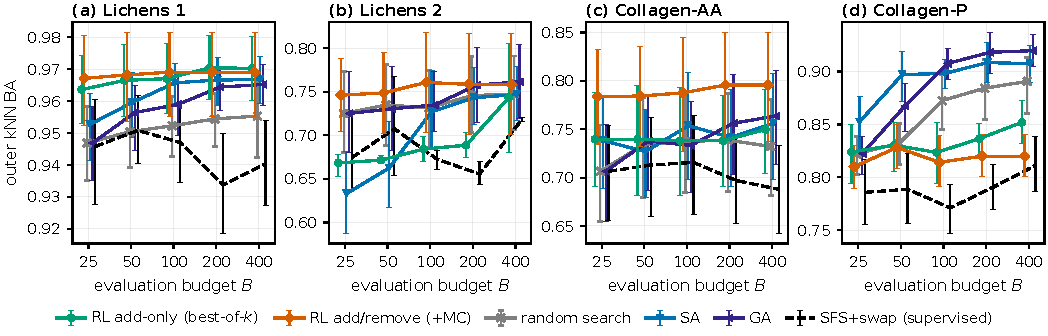
\includegraphics[width=\textwidth]{figures/fig_fewshot.pdf}
\caption{Few-shot search on the target (S3, $n=8$): outer kNN BA vs.\ the number of labelled objective evaluations $B$. RL policies are the leave-one-dataset-out policies transferred to the target; mean and 95\% CI over folds and seeds.}
\label{fig:fewshot}
\end{figure*}

\begin{figure*}[t]
\centering
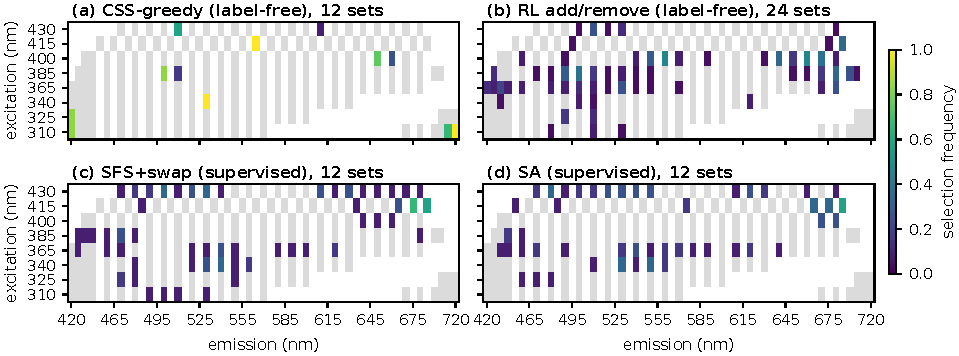
\includegraphics[width=\textwidth]{figures/fig_eem_pairs.pdf}
\caption{Selection frequency of excitation--emission pairs on Lichens1 ($n=8$) over all outer folds and repeats; grey cells are admissible pairs never selected.}
\label{fig:eem}
\end{figure*}

\textbf{Few-shot search (S3, Fig.~\ref{fig:fewshot}, Table~\ref{tab:fewshot}).} When a few labelled evaluations are allowed on the target, the transferred policy is a strong prior: with only $B=25$ evaluations both RL variants match SA (pooled differences $+0.007$ and $0.000$, n.s.) and the add/remove policy with look-ahead gives the best accuracy at every budget on Lichens1, Lichens2 (up to $B=100$) and Collagen-AA, where it also overfits less (lower inner $\JS$, higher outer BA). Classic search catches up as the budget grows; at $B=400$ SA is ahead by 0.017--0.024 (Holm $p=0.008$/$0.08$), driven by Collagen-P, where GA/SA reach 0.92 and the policy plateaus at 0.82--0.85. Look-ahead versus best-of-$k$ add-only differs by less than 0.008 (n.s.).

\begin{table}[t]
\centering
\caption{Few-shot search (S3), $n=8$: outer kNN BA for budgets $B$ of labelled evaluations on the target.}
\label{tab:fewshot}
\resizebox{\columnwidth}{!}{{\small
\setlength{\tabcolsep}{3pt}
\begin{tabular}{llcccccc}
\toprule
Dataset & $B$ & RL add (BoK) & RL add/rem (MC) & Random & SA & GA & SFS+swap \\
\midrule
Lichens-1 & 25 & 0.964 & \textbf{0.967} & 0.947 & 0.953 & 0.947 & 0.946 \\
 & 100 & 0.967 & \textbf{0.969} & 0.952 & 0.966 & 0.959 & 0.947 \\
 & 400 & \textbf{0.970} & 0.969 & 0.955 & 0.967 & 0.965 & 0.940 \\
\midrule
Lichens-2 & 25 & 0.668 & \textbf{0.746} & 0.725 & 0.633 & 0.725 & 0.674 \\
 & 100 & 0.684 & \textbf{0.761} & 0.731 & 0.727 & 0.735 & 0.673 \\
 & 400 & 0.743 & 0.758 & 0.747 & 0.747 & \textbf{0.761} & 0.719 \\
\midrule
Collagen (acetic) & 25 & 0.740 & \textbf{0.784} & 0.707 & 0.738 & 0.707 & 0.706 \\
 & 100 & 0.738 & \textbf{0.788} & 0.737 & 0.754 & 0.733 & 0.716 \\
 & 400 & 0.750 & \textbf{0.796} & 0.732 & 0.756 & 0.764 & 0.688 \\
\midrule
Collagen (pepsin) & 25 & 0.824 & 0.810 & 0.822 & \textbf{0.853} & 0.822 & 0.786 \\
 & 100 & 0.824 & 0.814 & 0.873 & 0.898 & \textbf{0.908} & 0.771 \\
 & 400 & 0.852 & 0.820 & 0.891 & 0.908 & \textbf{0.920} & 0.811 \\
\bottomrule
\end{tabular}
}
}
\end{table}

\begin{figure}[t]
\centering
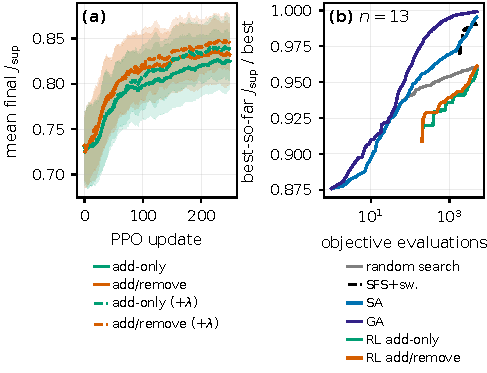
\includegraphics[width=\columnwidth]{figures/fig_training.pdf}
\caption{(a) PPO training curves (mean final $\JS$ of training episodes, mean and range over the six source pools): add/remove reaches its plateau earlier than add-only; dashed ($+\lambda$): with wavelength features. (b) S1 anytime curves at $n=13$: best-so-far $\JS$, normalised per task by the best value found by any method.}
\label{fig:training}
\end{figure}

\textbf{Is the reversible policy harder to train?} No. Despite the longer episodes and the delayed credit of a swap, add/remove policies reach within 0.01 of their final training return after 112--123 PPO updates versus 153--166 for add-only (Fig.~\ref{fig:training}a), with a comparable final value (0.834 vs 0.829 without, 0.837 vs 0.839 with wavelength features). Paired credit for the remove--add cycle, the tabu mask and the \stp{} action keep the refinement stable.

\textbf{Which pairs, and at what hardware cost?} Fig.~\ref{fig:eem} shows that label-free CSS returns almost the same few pairs in every fold, whereas the reversible policy and the supervised searchers spread their choices over more excitations, mostly 365--430\,nm, and over the short- and long-wavelength ends of the emission range. Adding a cost $\mu$ per distinct excitation to the reward reduces the number of light sources from 5.3 to 1.0 for the RL policy (4.8 to 1.5 for SA) while kNN BA on Lichens1 stays at 0.93--0.97.



\section{Discussion and conclusion}
The study answers the question that motivated it with a qualified yes. The ability to remove and swap pairs makes a transferred selection policy consistently better than an otherwise identical add-only policy, by 2--3 BA points on average and up to 6 points, and the advantage is largest when the policy meets a sample type unlike its training data. This supports the intuition that undo actions matter most where a constructive policy is miscalibrated~\cite{barrett2020eco}. The reversible policy was not harder to train: shared swap credit, tabu masking and a stop action made refinement converge in fewer updates than construction.

Three negative results are equally important for practice. First, when the selection objective can be evaluated cheaply on the target, RL is not the right tool: SA and GA find better subsets at the same budget, and they reach the certified optimum at $n=3$. Second, the inner objective overfits few specimens, so strong search buys little on held-out specimens; reporting the inner--outer gap should be standard. Third, a label-free greedy column-subset rule is a strong baseline that most published band selectors do not report; a learned policy should be judged against it. Using the policy to refine that greedy set is safe, because it mostly stops, but it paid off on only one of four targets. Wavelength-position features hurt transfer, which suggests that what transfers between sample types is a statistical selection rule, not a spectral prior.

\textbf{Limitations.} We had four datasets from two sample families and one instrument, so the source pools for transfer are small (two or three datasets); task augmentation by class subsets and excitation dropout only partly substitutes for more acquisitions. Specimen counts are low (three per class for collagen), which makes every outer estimate noisy. Simulation-based training, for example in a physics-based simulator, and sequential acquisition where the policy controls the instrument are natural next steps.

\textbf{Conclusion.} Reversible add/remove/stop actions are a simple, robust improvement for RL-based spectral pair selection on new data, but classic search should remain the default for a fixed labelled dataset, and label-free greedy selection is the baseline to beat. % TODO(authors): code-availability statement.

\bibliographystyle{IEEEtran}
\bibliography{refs}
\end{document}
